\section{Introduction}
\label{sec:introduction}
In this laboratory we synthesize and measure the superconductivity of yttrium barium copper oxide
(YBCO). In contrast to many other superconducting materials it is a high $T_C$
superconductor, denoting that its superconducting phase can be reached by cooling it with liquid
nitrogen. This has a cost advantage over low $T_C$ superconductors which require helium cooling to
operate.

\subsection{Superconductivity}
\label{sec:Superconductivity}
A superconductor is a material with a critical behavior at a temperature $T_C$, below which the
electrical resistance $\rho$ drops to an order of $10^{-21} - 10^{-22} \Omega / \text{cm}$, as it is shown
in \autoref{fig:sample_cond}. 

The existence of superconductivity is not only bound to the temperature $T<T_C$, but also to a
critical magnetic field $H < H_C$. An important distinction here is between type-I and type-II
superconductors, which will be covered more in detail in \autoref{sec:intr:meissner}.

\begin{figure}
  \centering
  \includegraphics[width=0.4\textwidth]{build/conductivity_example.pdf}
  \caption{Sample plot for the conductivity of a superconductor.}
  \label{fig:sample_cond}
\end{figure}

\subsection{Meissner-Ochsenfeld effect}
\label{sec:intr:meissner}
% repelling of magn. fields
Apart from the low electrical resistance, superconductors can also be characterized by their perfect
diamagnetism, i.e. it expels an external magnetic field. 

While a type-I superconductor always maintains the diamagnetism as long as $T < T_C$ and $H < H_C$, a type-II
superconductor has two critical magnetic field densities $H_{C1}$ and $H_{C2}$. For $H < H_{C1}$ a
type-II semiconductor has perfect diamagnetism, but for $H_{C1} < H < H_{C2}$ the external magnetic
field can enter the material, eventhough the superconductivity (low $\rho$) is
maintained.

A consequence of the perfect diamagnetism is that permanent magnets can levitate on superconductors.
For a given YBCO sample and a neodymium magnet this is shown in \autoref{fig:intr:meissner}.

\begin{figure}
  \centering
  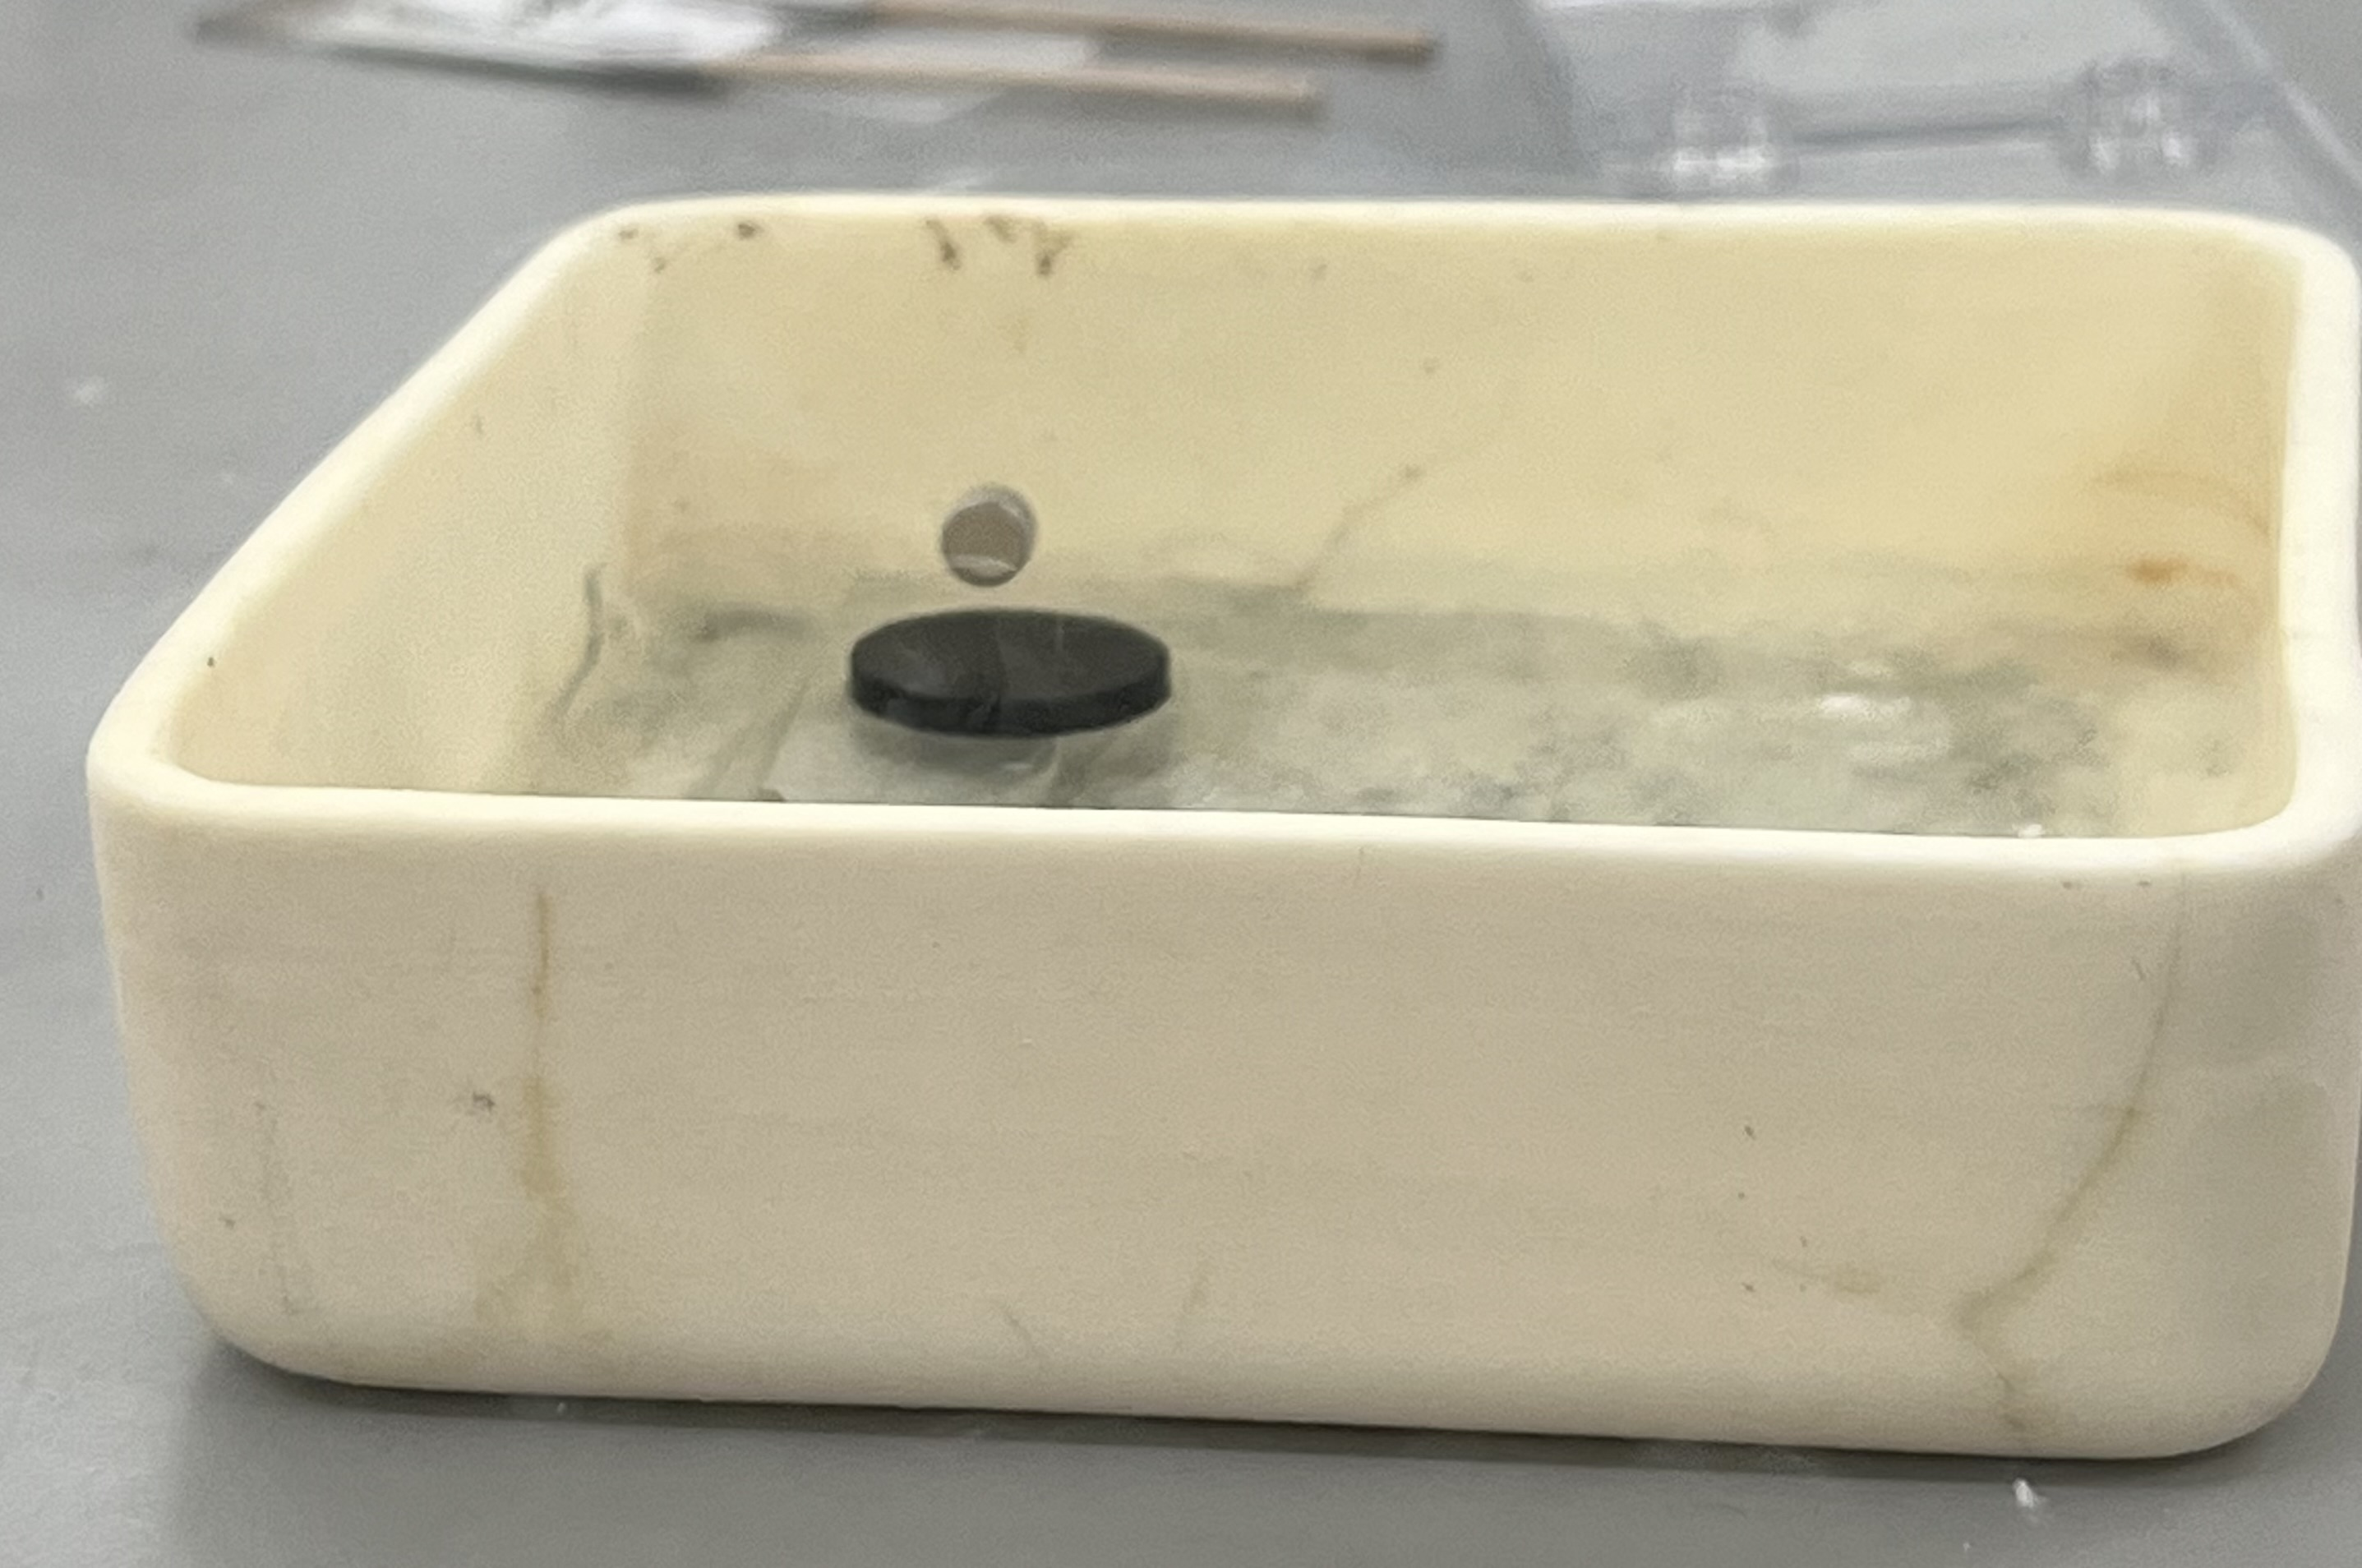
\includegraphics[width=0.4\textwidth]{media/meissner.jpg}
  \caption{A neodymium magnet floating on superconducting YBCO due to the repelling of magnet field
  (Meissner effect). The YBCO sample has been given to our group by the lab supervisor.}
  \label{fig:intr:meissner}
\end{figure}

